% Figure 4: Feature Engineering and Target Leakage Mechanism
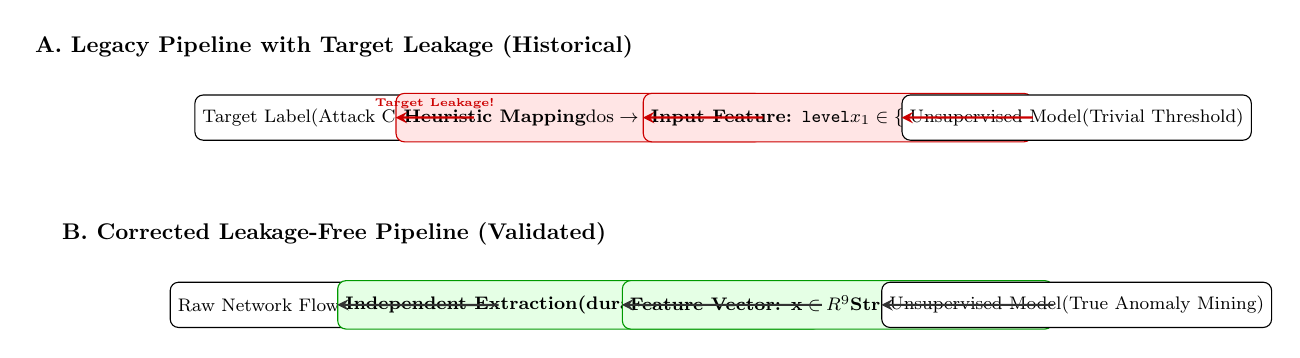
\begin{tikzpicture}[
    scale=0.82, every node/.style={transform shape},
    box/.style={rectangle, draw=black, rounded corners=3pt, fill=white, minimum width=2.5cm, minimum height=0.7cm, text centered, font=\footnotesize},
    warnbox/.style={rectangle, draw=red!80!black, fill=red!10, rounded corners=3pt, minimum width=2.8cm, minimum height=0.75cm, text centered, font=\footnotesize\bfseries},
    okbox/.style={rectangle, draw=green!60!black, fill=green!10, rounded corners=3pt, minimum width=2.8cm, minimum height=0.75cm, text centered, font=\footnotesize\bfseries},
    arrow/.style={thick,-stealth,draw=black!80},
    warnarr/.style={thick,-stealth,draw=red!80!black}
]

% Legacy Leaked Path
\node at (0, 2.5) {\textbf{A. Legacy Pipeline with Target Leakage (Historical)}};

\node [box] (raw_label) at (0, 1.4) {Target Label\\(Attack Category)};
\node [warnbox] (leak_map) at (3.8, 1.4) {Heuristic Mapping\\$\mathrm{dos} \to 13, \mathrm{norm} \to 2$};
\node [warnbox] (feat_lvl) at (7.8, 1.4) {Input Feature: \texttt{level}\\$x_1 \in \{2, 8, 10, 13, 14\}$};
\node [box] (model_leak) at (11.5, 1.4) {Unsupervised Model\\(Trivial Threshold)};

\draw [warnarr] (raw_label) -- node[above, font=\tiny\bfseries, text=red!80!black] {Target Leakage!} (leak_map);
\draw [warnarr] (leak_map) -- (feat_lvl);
\draw [warnarr] (feat_lvl) -- (model_leak);

% Corrected Leakage-Free Path
\node at (0, -0.4) {\textbf{B. Corrected Leakage-Free Pipeline (Validated)}};

\node [box] (raw_packet) at (0, -1.5) {Raw Network Flow\\\& Packet Headers};
\node [okbox] (stat_extract) at (3.8, -1.5) {Independent Extraction\\(duration, bytes, errors)};
\node [okbox] (feat_clean) at (7.8, -1.5) {Feature Vector: $\mathbf{x} \in \mathbb{R}^9$\\Strictly Operational};
\node [box] (model_clean) at (11.5, -1.5) {Unsupervised Model\\(True Anomaly Mining)};

\draw [arrow] (raw_packet) -- (stat_extract);
\draw [arrow] (stat_extract) -- (feat_clean);
\draw [arrow] (feat_clean) -- (model_clean);

\end{tikzpicture}
